\chapter{Related work} \label{chap:related_work}
In this chapter, we will go in-depth discussing common approaches that are being used in the group recommendation task. First, specifying the main approaches, dividing them into groups by how they approach the transition from single-user preferences to group results. Then mentioning the main simple techniques and describing how they interact with the common recommendation approaches. And at last diving into some of the more advanced methods that optimize the aggregation in a more elaborate way.

\section{Categories} \label{sec:03_categories}
We assume that we have individual user preferences (if group preferences are available, then the task actually becomes a simple recommendation with the group acting as a single user), therefore it is necessary to make a distinction based on where the algorithm goes from the preference of the group's individual users to a result for the whole group.

We can put each algorithm into one of the following three groups based on the aggregation step:
\begin{itemize}
    \item \textbf{Aggregate models} \newline
    The aggregation works on merging the preferences of each member of the group into a single set of preferences that can be then directly consumed by a recommender system, therefore creating a group preference model. Aggregating the single-user preferences either directly by aggregating ratings of seen, or and rated items, or by aggregating the extracted models of user preference to create a single model for the whole group, such as preference matrix in matrix factorization approaches, text descriptions, or item-based recommendations and so on, we will discuss these techniques later.
    
    % Aggregates the models for RS. Recommender is working on a set of already aggregated group preferences, either directly aggregating ratings of seen items, or more high level extracted features such as preference matrix in matrix factorization approaches, text description for item-based recommendations and so on, we will discuss these techniques later.
    
    This aggregation step precedes the recommendation step. We can see a visualization on Figure \ref{fig:before_rec_agg}.
    
    
    \item \textbf{Aggregate predictions} \newline
     Aggregates predictions outputted from RS. Recommender recommends separately for each member of the group based solely on their single-user preferences. Then the resulting recommended items are aggregated together to a single list of recommendations for the whole group. There are two main ways how the final list can be created. Either directly take items recommended to each user and append them together in some specified manner, or the second way, calculate some common utility function from all recommended items and select those that are the most fitting to the group based on this utility function. We will discuss both in more detail in \ref{sec:03_simple_aggregation_metods}.
     
     The aggregation step follows after the actual recommendation step. We can see a visualization of this approach on Figure \ref{fig:after_rec_agg}.
     
    \item \textbf{Aggregation is a uniform part of the recommender} \newline
    In this case, the algorithm directly works with users of the group and does not allow for a clear distinction of the aggregation step. It is deeply and inseparably built into the algorithm itself. Sometimes the perception of the inseparability of these two steps can vary in the literature. Some could say that for example aggregating the user profiles in matrix factorization makes the aggregation inseparable, because there is a specific preprocessing done before the aggregation step. But others will point out, that the user latent matrix is just a representation of a user preference, even if processed by the algorithm itself. We will let the reader decide for themselves where they see the distinguishing border. We will briefly discuss the available methods in \ref{sec:03_advanced_methods}
\end{itemize}


This presented grouping based on the aggregation step is different from the main literature  \cite{recommendations_to_groups-jameson2007} and \cite{grouprecommendersystems_felfernig2018group}, where they also make a distinction into three groups, but instead based on the data that the aggregation processes and the position. Instead we have chosen a little different distinction based more on interaction of the aggregation with the recommender system, essentially putting two groups from aforementioned literature under single group (\textit{aggregate models}), but with the mentioned possible subdivision.
    

\begin{figure}[htbp]
    \centering
    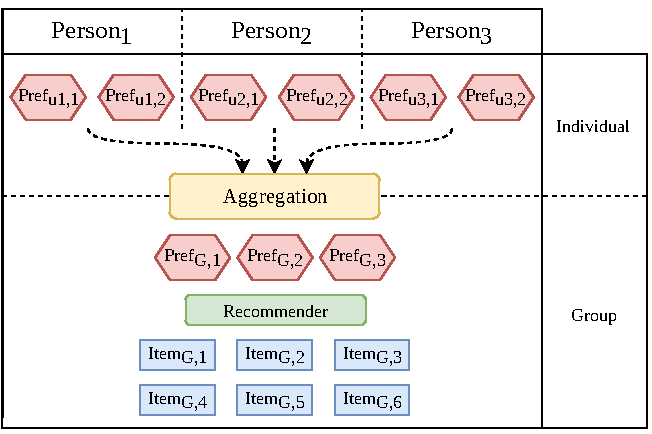
\includegraphics{img/before-rec-aggregation.pdf}
    \caption{High level overview of group recommendation with aggregation of individuals' preferences, before recommendation.}
    \label{fig:before_rec_agg}
\end{figure}

\begin{figure}[htbp]
    \centering
    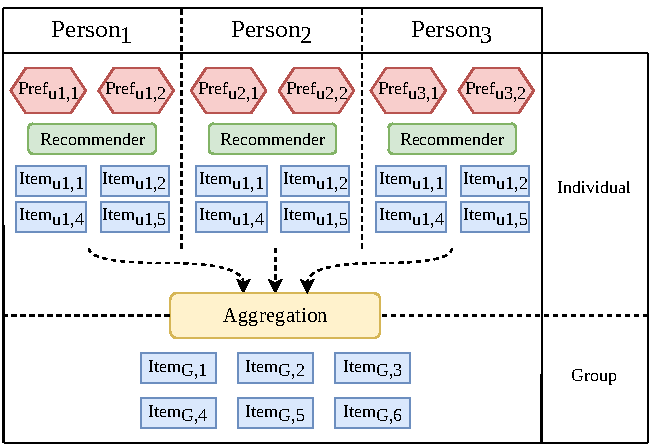
\includegraphics{img/after-rec-aggregation.pdf}
    \caption{High level overview of group recommendation with aggregation on top of recommendation results for individual users.}
    \label{fig:after_rec_agg}
\end{figure}






\section{Simple aggregation methods}\label{sec:03_simple_aggregation_metods}
We will now introduce the main aggregation functions (interchangeably as "aggregation strategies", "aggregation methods") used, together with an overview of how they interact with the single-user recommender systems introduced in \ref{subsec:01_rec_sys.main_alg_approaches}
\subsection{Methods}\label{subsec:03_simple_aggregation_methods.methods}

The main aggregation methods can be divided into three groups, based on their high-level approach into - majority, consensus, and borderline based strategies. The majority-based generally use the most popular item among the group members, the consensus-based consider preferences of all the group members, and the borderline-based consider a subset of the items by some limiting criteria.

We now list the most common aggregation methods as mentioned in \cite{grouprecommendersystems_felfernig2018group}, \cite{masthoff_2011_group_rec_systems} and \cite{masthoff_2004_group_modeling} specify to which of the group mentioned above they belong.
%The common aggregation methods as mentioned in \cite{grouprecommendersystems_felfernig2018group}, \cite{masthoff_2011_group_rec_systems} and \cite{masthoff_2004_group_modeling} are:

\begin{itemize}
    \item \textbf{Additive utilitarian} (ADD, consensus)\newline
        Sum of scores for an item across the group
        \begin{equation}
            \argmax_{i \in I}{\sum_{u \in G}{\textrm{score}(u,i)}}
        \end{equation}
    
    \item \textbf{Approval Voting} (APP, majority)\newline
        Number users that like the item above a certain threshold
        \begin{equation}
            \argmax_{i \in I}{
                \big\lvert{\left\{
                    u \in G : \textrm{score}(u,i) \geq \textrm{treshold}
                \right\}}\big\rvert
            }
        \end{equation}
    
    \item \textbf{Average} (AVG, consensus)\newline
        Average of scores for an item across the group
        \begin{equation}
            \argmax_{i \in I}{\dfrac{\sum_{u \in G}{\textrm{score}(u,i)}}{\abs{G}}}
        \end{equation}
    
    \item \textbf{Average without Misery} (AVM, consensus)\newline
        Average of scores for an item across the group only if the item is above a certain threshold for all group members
        \begin{equation}
            \argmax_{ i \in I : \nexists u \in G | \textrm{score}(u,i) \leq \textrm{treshold}}{
                \dfrac{\sum_{u \in G}{\textrm{score}(u,i)}}{\abs{G}}
            }
        \end{equation}
        
    \item \textbf{Borda count} (BRC, majority)\newline
        Sum of scores derived from item rankings. The ranking score is defined for each user by ordering the user's items by score and awarding points corresponding to the location of the item in this ordered list. Worst item receiving 1 point and best item $|I|$ points.
        \begin{equation}
                \argmax_{i \in I}{\left(\sum_{u \in G}{\textrm{RankingScore}(u,i)}\right)}
            \end{equation}
        Where \textit{ranking score} is defined as follows:
        \begin{equation*}
            \textrm{RankingScore}(u,i) := 
            \big\lvert{\left\{
                i_{other} \in I : \textrm{score}(u,i_{other}) \leq \textrm{score}(u,i)
            \right\}}\big\rvert
        \end{equation*}
    
    \item \textbf{Copeland rule} (COP, majority)\newline
        Difference between number of wins and losses for pair-wise comparison of all items
        \begin{equation}
            \argmax_{i \in I}{
                \big(\textrm{W}(t, I - t) - \textrm{L}(t, I - t)\big)
            }
        \end{equation}
    
    \item \textbf{Fairness} (FAI, consensus)\newline
        Users, in turn, one after another select their top item.
        \begin{equation}
            \argmax_{i \in I}{{\textrm{score}(u_{current},i)}}
        \end{equation}
        Where $u_{current}$ is user selected from $G$ for each iteration according to some (in most cases circular, or ping pong) rule.
    
    \item \textbf{Least misery} (LMS, borderline)\newline
        Uses the lowest received rating among the group members as the item's aggregated rating.
        \begin{equation}
            \argmax_{i \in I}{\left(\min_{u \in G}{\left(\textrm{score}(u,i)\right)}\right)}
        \end{equation}
    
    \item \textbf{Most Pleasure} (MPL, borderline)\newline
        Uses the highest received rating among the group members as the item rating.
        \begin{equation}
            \argmax_{i \in I}{\left(\max_{u \in G}{\left(\textrm{score}(u,i)\right)}\right)}
        \end{equation}
        
    \item \textbf{Majority Voting} (MAJ, majority)\newline
        Uses the rating that was given by the majority of the group's members. (Can only work on discrete ratings)
        \begin{equation}
            \argmax_{i \in I}{\left(\mode_{u \in G}{\left(\textrm{score}(u,i)\right)}\right)}
        \end{equation}
    
    \item \textbf{Most Respected Person} (MRP, borderline)\newline
        Uses rating proposed by the most respected member of the group.
        \begin{equation}
            \argmax_{i \in I}{\textrm{score}(u_{most\_respected},i)}
        \end{equation}
        
        
    \item \textbf{Multiplicative} (MUL, consensus)\newline
        Multiplies all received ratings together.
        \begin{equation}
            \argmax_{i \in I}{\left(\prod_{u \in G}{\textrm{score}(u,i)}\right)}
        \end{equation}
        
        
    \item \textbf{Plurality Voting} (PLU, majority)\newline
        Each user has a set number of votes that get distributed. The item with the most received votes is selected.
        \begin{equation}
            \argmax_{i \in I}{\left(\sum_{u \in G}{\textrm{VotesAwarded}(u,i)}\right)}
        \end{equation}
        
        Where \textit{votes awarded} is some function that decides for each user how the available votes will be distributed among the items.
        
\end{itemize}

Some of the methods have an additional distinguishing factor, which is that they are iterative calculations instead of a single calculation that returns the final ordering. Most notably \textit{Fairness}, it calculates the next item purely from a currently selected user, users changing in iterations one after another. Another one is \textit{Plurality Voting}, this technique can also be iterative but it is not mandatory. Where after the top item is selected we reset the calculation, therefore selecting top items in an iterative manner. All the other ones are single-iteration methods, where the final list requires only one calculation.

Now we will show how these strategies work together with a recommendation in order to provide a full group recommender system, which will serve as an introduction of the inner workings of such system in order for us to then continue towards more advanced aggregation methods.

\subsection{Usage with recommender systems}
We now need to distinguish between \textit{model aggregation} and \textit{prediction aggregation} due to in most cases very different inputs and required outputs from the aggregation.
\subsubsection{Prediction aggregation}
In most cases using them as \textit{prediction aggregation} after the recommendation is quite straightforward. In all (to us known) cases RS returns recommended items together with some sort of rating of the recommendation. There are some applications where this presumption does not hold, such as building a group recommendation aggregation on top of a \textit{black box} recommender that only returns a list of items, for example, if extracting recommended items data from a web page where we only retrieve the list itself and we do not have access to the underlying recommender system. But in the following section we will assume that we have a full access to the rating data of the outputted items. We further assume that if necessary we can acquire ratings and ordering for all possible items.

As shown on Figure \ref{fig:after_rec_agg}, we first get a list of recommended items (together with ratings) for each user. Then we can directly apply the methods mentioned in \ref{subsec:03_simple_aggregation_methods.methods}.

\subsubsection{Model aggregation}
Running aggregation on top of user preferences, instead of lists of recommended items is more challenging due to many possible inputs that the recommender can take, such as explicit or and implicit feedback. As discussed in section \ref{sec:03_categories}, we have two main options, aggregation of ratings and aggregation of mined preferences.

First, the aggregation of ratings, in other words creating a set of ratings that represent the whole group. This approach is preferred due to its simplicity. We can use many of the before mentioned simple methods, mainly the \textit{consensus-based} which aggregate ratings directly (positive as well as negative ratings). Other mentioned methods can be used as well, but some of them do not make much sense to adapt, for example, the voting-based, with which we will be very limited due to the usual sparsity of the feedback ratings that we have available.

The second option, the aggregation of mined preferences, is more present in content-based systems. Where we aggregate not the rating themselves but some other data that represent the users' likes and dislikes. As an example, we will use the \textit{tf-idf} keyword extraction which is by far the most popular method used in the text-based recommendation as mentioned in \cite{beel_2016_rs_literature_survey}. We can weight \textit{tf-idf} concepts extracted from the user feedback by the received rating, and then aggregate these concepts together for the whole group. As we can see, it is a little more elaborate approach that requires more modifications to the simple methods mentioned.

%The above mentioned aggregation methods can be used with collaborative filtering, mentioned in \ref{subsec:01_group_rec_sys.common_aproaches}, as a \textit{model aggregation method} (Fig. \ref{fig:before_rec_agg}) as well as a \textit{prediction aggregation method} (Fig. \ref{fig:after_rec_agg}). As already mentioned the method is based on the idea of recommending items that were liked by users with similar preference. First we mention how \textit{prediction aggregation} works with collaborative filtering.

%\section{Advanced aggregation methods}\label{sec:03_advanced_aggregation_methods}
\section{Advanced methods}\label{sec:03_advanced_methods}
As we can see, the simple methods mentioned before are quite straightforward, they have mostly very simple and clear objectives, and try to optimize in different ways some quite vaguely specified goal. But as we have discussed in \ref{chap:fairness}, the objective is quite hard to define and measure. We will now introduce some other methods that either directly or indirectly try to optimize some better-specified goal.

\subsection{GFAR} \label{subsec:03_advanced_methods.gfar}
So far we have introduced methods that do not directly specify any form of optimization in a direction of \textit{fairness}. A new method introduced in\cite{GFAR-kaya2020} directly optimizes the resulting list to balance the relevance of the recommended items in a rank-sensitive way.

\subsubsection{Introduction}

As mentioned they focus on the \textit{fairness} of top-$N_G$ (\textit{fairness} of the top N recommended items for the group G). Where they define \textit{fairness} as a property of the top-$N_G$ items, not just any single item but the whole list. As already discussed in \ref{sec:01_rec_sys} the difference between optimization independently item after item versus in some way for the whole list can yield significantly better results when it comes to sequential consumption of items or and balancing users with different preferences. For example, being one member of the group being treated unfairly due to different preferences from the rest of the group, then fairness defined as a property of the whole list can in some way compensate and give more priority for balancing fairness forwards this one user. This kind of unfairness is the main problem that they try to solve.

We have already mentioned one algorithm that tries to balance fairness of the whole list in \ref{subsec:03_simple_aggregation_methods.methods}, FAI, which generates the aggregated results in iterations, each iteration optimizing for a different user in turns. This approach solves the aforementioned problem in a very simple (although somewhat dull) way by not considering the group preferences at all and just trying to please everyone in turns not considering if the item will be liked by the rest of the group.


\subsubsection{Approach}

What if we have instead taken into account the previously recommended items when we are selecting the next one in the list? The authors propose defining \textit{fairness} together with ordering within the group by saying that "a top-$N$ is fair to a group if the relevance of the items is balanced across the group members for \textit{each prefix} of the top-$N_G$". In other words for each iteration, we try to select an item that improves the balance as much as possible.

Let us first define Borda relevance following \cite{xiao_2017_fairness_aware_g_rec} as:


% In original paper there is an error in the direction of </>
\begin{equation}
    \textrm{Borda-rel}(u,i) = 
    \big\lvert{
        \left\{j : \textrm{rank}(j, \textrm{top-}N_u) < \textrm{rank}(i, \textrm{top-}N_u) \right\}, \forall_j \in \textrm{top-}N_u)
    }\big\rvert
\end{equation}

Where rank is the position of item $i$ in the user's $u$ candidate list (position is determined by ordering the items based on the returned items score, from the best to the worst). Borda relevance essentially gives zero points to the last item and increases the points by one for each position up in the list, with the first/top item getting $(\#\textrm{items} - 1$) points.

Now we can set probability of item $i$ being relevant for user $u$ as:

\begin{equation}
    p(\textrm{rel}|u, i) = \frac{\textrm{Borda-rel}(u, i)}{\sum_{j \in \textrm{top}-N_u}{\textrm{Borda-rel}(u, j)}}
\end{equation}

Let also $p(\neg\textrm{rel}|u, S)$ be the probability that item $i$ is not relevant for any of the items in set $S$. We derive the probability that atleast one item from set $S$ is relevant to the user $u$ as:

\begin{equation} \label{eq:atleast_one_relevant}
\begin{aligned}
    p(\textrm{rel}|u, S) &= 1 - p(\neg\textrm{rel}|u, S) \\
    & = 1 - \prod_{i \in S}{(1 - p(\textrm{rel}|u, i))}
\end{aligned}
\end{equation}

Now we want to generalize for the whole group, so we define $f(S)$ as the sum of probabilities for each user that they find at least one relevant item in the set $S$:

\begin{equation} \label{eq:relevance_for_set}
\begin{aligned}
    f(S) &= \sum_{u \in G}{\left(1 - p(\neg\textrm{rel}|u, S)\right)} \\
    & = \sum_{u \in G}{\left(1 - \prod_{i \in S}{(1 - p(\textrm{rel}|u, i))}\right)}
\end{aligned}
\end{equation}

We have used the Group G as a constant in equation \ref{eq:relevance_for_set} and forward, the group will stay the same during the calculation. $f(S)$ shows how to balance the fairness amongst the group members for a specified set of item. We now want to extend it in order to make it rank-sensitive by defining a marginal gain in function $f$ for adding a new item $i$ to the set $S$ as follows:

\begin{equation} \label{eq:relevance_for_set_add}
\begin{aligned}
    f(i, S) &= f(S \cup {i}) - f(S) \\
    & = \sum_{u \in G}{\left[p(\textrm{rel}|u, i) \prod_{j \in S}{(1 - p(\textrm{rel}|u, j))}\right]}
\end{aligned}
\end{equation}

Where we have used equations \ref{eq:atleast_one_relevant} and \ref{eq:relevance_for_set}. And finally, we can define an ordered set that is considered fair if it balances each of its prefixes. In other words, the first item of the set should be considered fair/balanced by all group members as much as possible, then the first two items and so on, we define fairness in an ordered set $OS$ as:

\begin{equation}
    \textrm{fair}(OS) = \sum_{k=1}^{|OS|}{f(OS)[k], \{i \in OS : \textrm{rank}(i, OS) < k\})}
\end{equation}


\subsection{Package-to-Group Recommendations}
Paper \cite{serbos_2017_fairness_packages_to_group_rec}?


\subsection{Top-N group RS with fairness}
Paper \cite{sacharidis_2019_top_n_with_fairness}?